% Report section types:  \part{}, \chapter{}, \section{}, \subsection{}, \subsubsection{}, \paragraph{}, \subparagraph{}.
% Article section types: \part{}, \section{}, \subsection{}, \subsubsection{}, \paragraph{}, \subparagraph{}.
\documentclass{article}
\usepackage{graphicx}
%\documentclass{report}
%\usepackage{fontspec}
\usepackage{hyperref}
%\setmainfont[Ligatures=TeX]{TeX Gyre Bonum}
%\setsansfont[Ligatures=TeX,Scale=MatchLowercase]{Latin Modern Sans}
%\setmonofont[Scale=MatchLowercase]{Inconsolata}
%\setmainfont[Numbers=Lining]{TeX Gyre Pagella}
\usepackage{lmodern}
\linespread{1.1}% spread lines out a little
\frenchspacing % remove extra space after punctuation
\begin{document}
\title{\textbf{oscaar}: Open Source Differential Photometry Code for Amateur Astronomical Research}
\author{Brett Morris}
\maketitle
\tableofcontents
%\setcounter{tocdepth}{1}
\section{Introduction}

\newcommand{\oscaar}{$ \mathtt{oscaar}$\ }
\newcommand{\code}[1]{\texttt{#1}}
\newcommand{\init}{\code{init.par}\ }

\oscaar is a differential photometry package built for users at observatories of any size and users of any experience level. The process of differential photometry can be applied to many astrophysical phenomena including transiting extrasolar planets, variable stars, rotating asteroids and more, and this code is prepared for any such use. 

The code was first designed in the summer of 2011 to take a series of CCD images obtained at the University of Maryland Observatory and churn out light curves of transiting extrasolar planets. If you're looking to do something similar, you've found the right code! The core of the code is written in Python, but it has been designed for users who have never seen Python before. That being said, experienced programmers will find that the guts of \oscaar provide a great toolkit for even the most demanding of photometric measurements.

Here we summarize the contents of this documentation. If you are new to photometric measurements, you may consider reading Section \ref{sec:collectingData}, which will summarize observing techniques to make successful photometric measurements. In Section \ref{sec:run}, we will detail how to run \oscaar from the graphical user interface (GUI) or other ways without directly coding in Python. In Section \ref{sec:api} we discuss the classes and methods that are built into \oscaar that users with programming experience may find useful to design their own analysis tools. 

\subsection{System Requirements} \label{sec:systemRequirements}

This software package runs on the following required software and modules:  \\ \\
\noindent
\indent \href{http://www.python.org/getit/}{\textbf{Python 2.7.1}}: The main language this software is written in \\
\indent \href{http://new.scipy.org/download.html}{\textbf{NumPy 1.6.0-py2.7}}: A Python module for efficient numerical computations \\
\indent \href{http://www.stsci.edu/resources/software_hardware/pyfits/}{\textbf{PyFITS 2.4.0}}: A Python module for FITS handling \\
\indent \href{http://matplotlib.sourceforge.net/index.html}{\textbf{Matplotlib 1.0.0-py2.7}}: A Python module for plotting\\
\indent \href{http://hea-www.harvard.edu/RD/ds9/}{\textbf{SAO Image DS9}}: A standard astronomical FITS display interface \\
\indent \href{http://www.wxpython.org/download.php#stable}{\textbf{wxPython}}: A Pythonic GUI toolkit


\subsubsection{Disclaimer}

Though the modules used in this package have been stable historically and probably will not go away any time soon, the \oscaar Team does not take any responsibility for problems that arise as a result of changes to future versions of these modules. Sorry!

\section{Collecting Data} \label{sec:collectingData}
\subsection{Telescope Tracking}

Differential photometry is generally done on a series of images of the same patch of the sky over a long period of time. You'll need a telescope that is well polar-aligned so that the telescope's tracking keeps the stars in nearly the same spot on your detector throughout the duration of your observations. It is an unreasonable challenge to align most small telescopes well enough to track a star perfectly over several hours, so \oscaar is built to monitor and correct for the drift in star positions on the detector over time. Just make sure your object of interest and a few comparison stars stay in the field throughout the whole observation. 

The star tracking algorithm follows each star individually over time. If your photometric target is an asteroid, for example, that moves relative to the comparison stars over time, \oscaar will happily track the asteroid and the comparison stars independently. There is one major weakness in \oscaar's tracking -- if you stop an observing run and start again with the stars in different positions on the detector, \oscaar will likely barf. If the stars move significantly (tens of pixels) between two adjacent exposures, you must run \oscaar separately on each half of the time-series.

\subsection{Defocusing} \label{sec:defocusing}

In precision photometry, relying on individual pixels is dangerous. Pixel defects occur frequently that can cause a pixel to read much higher counts than they actually receive (these are called ``hot pixels'') or sometimes much lower counts (``dead pixels''). If your target object is perfectly focused on a few pixels, you may be putting all of your photometric-eggs in one basket. Thus it is often advised that you \textbf{do not focus the telescope perfectly} when doing photometric measurements. If you can, defocus the telescope significantly so that you spread out the starlight over a few of pixels, and your pixel-to-pixel variations will play a less-significant role in the introduction of unwanted systematic noise and bias. 

Some photometry codes prefer objects focused in Gaussian-like shapes, but \oscaar is written to accurately track stars of unconventional shapes. At the University of Maryland Observatory, we make most of our measurements on a 6in refractor. We defocus the stars until they look like small donuts (the hole is an artifact of the optical path of the refractor), and we've found that our photometry comes out best this way. \oscaar won't complain if your stars are donut-shaped, Gaussian or somewhere in between.

One must keep in mind that by spreading out the light over many pixels, the counts measured by each pixel is lower. As a result, defocusing is most helpful when observing bright objects. If the source you are observing is bright enough, you can defocus significantly without losing too much signal. However, it is important to note that the quality of your light curve will be directly related to how much more signal than noise you detected. Use defocusing sparingly (or not at all) when imaging dim targets.

\subsection{Theory: Photon Noise}

There is a fundamental physical limit to the signal-to-noise ratio that can be achieved in photometric measurements. Since photometry is the process of counting photons, there is a type of statistical uncertainty introduced into each measurement that goes by many names: \textit{photon noise, Poisson uncertainty, shot noise,} etc. This uncertainty is unavoidable in counting measurements and is easy to calculate -- the photon noise, or the uncertainty in a measurement of $N$ photons, $\sigma_N$ is

\begin{eqnarray}
\sigma_N = \sqrt{N}. \label{eqn:photonNoise}
\end{eqnarray}

\noindent You can see directly from Equation \ref{eqn:photonNoise} that the fractional uncertainty in the signal ($\sigma_N/N$) decreases with increasing $N$ as $1/\sqrt{N},$
so the more signal you have, the lower the limiting fundamental uncertainty. Of course, in practice there are many additional noise sources that will add uncertainty into your data and increase the scatter in your light curves. 
 
\subsection{Dark Fields and Flat Frames}

Collecting dark frames and flat fields is standard practice for removing systematic effects from CCD images. Flat fields correct for dust and other inconsistencies in the optical path artificially brighten or dim the objects that you image. Dark frames remove some flaws in the CCD like hot pixels and dark current variations. Some CCD imaging software like MaxIm DL have easy preset routines for taking dark frames. Collecting good flat fields can sometimes be more of an art than a science, but good flats are important for good photometry. We recommend taking $\sim8$ dark frames and flat fields for each set of observations you take. \oscaar will take the mean of these sets and apply them appropriately to each image of your data set. 

\subsection{Picking A Target}
\subsubsection{Transit Predictions}
So you're planning a night of transiting extrasolar planet observations, and you need to know what planets are transiting in your part of the world. We recommend using the \href{http://var2.astro.cz/ETD/predictions.php}{Czech Astronomical Society Exoplanet Transit Database's Transit Prediction tool}. If you enter your latitude and longitude, this web-tool will tell you which bright transiting extrasolar planets will be visible and transit on a given night from your location. This tool is invaluable for planning. It's also great because you can contribute to this database by submitting your light curves to help constrain the orbital parameters of the planets. With a telescope and \oscaar, you can contribute to real science!

\subsubsection{Choosing The Field}
When you chose your target for differential photometry, you need to be sure there are other stars in the imaging field. Here we'll define some terms that are important from here on:  \\ 

\noindent \textbf{Target Star}: The target of your observations -- the host star to an exoplanet or the variable star that you're measuring for intrinsic variations in luminosity. Of course, this ``star'' could be an asteroid, too. \\\\
\textbf{Comparison Star}: A star other than the target star that you will use as a basis for determining the intrinsic variations in the brightness of the target star. The comparison star should be one that is not known to have intrinsic variations. \\

There must be at least one comparison star in order to do differential photometry, and the more the better. There is no magic number of comparison stars to have, but if you have the opportunity to fit more control stars in the field by rotating your CCD or effectively ``zooming out," it will be worth your while. Based on prior experience with \oscaar, $ \sim $10 good stars should do. Later, we'll discuss how to know which ones are ``good.''

Photometry of bright stars is always preferable to dim stars, but of course there are more dim stars than bright stars in most of the images you will take. In order to avoid uncertainty introduced noise with very dim stars, pick control stars with peak intensities more than double the average background intensity in the area surrounding the star. 

Different transiting exoplanets change the brightnesses of their host stars by different amounts. This parameter is called ``\textbf{depth}" and is often measured in units of millimagnitudes (mmag). The greater the depth of a transit, the more likely you will be capable to detect the transit. Since some of these depths are so small, it might is a good idea to perfect measuring \href{https://sites.google.com/site/aavsosppsection/}{short period pulsating (SPP) variable stars} with high amplitude luminosity oscillations (like \href{http://www.aavso.org/vsx/index.php?view=detail.top&oid=4356}{YZ Boo}) before you move on to exoplanets. Once you characterize your ability to measure the large intrinsic variations of variable stars, you will be able to characterize your ability to detect the small depth regime of transiting exoplanets. 

\subsection{Imaging Software}
A bunch of imaging packages could suite your needs for photometry with \oscaar. At the University of Maryland Observatory, we use \href{http://www.cyanogen.com/maxim_main.php}{MaxIm DL} to handle our imaging. Any imaging software that enables you to take a time-series of CCD images will do. 

Observing software like MaxIm DL allow you to choose your imaging \textbf{binning}, which enables the detector to read-out pixels in groups. For example, a $2\times2$ binning will take a square of four pixels and save them as one composite pixel. This reduces the read-out time, the size of the output files, and the run time of scripts that have to read and manipulate those images. We recommend that you use $2\times2$ binning when you can for these reasons. It is often unimportant to save images at the full-resolution of the detector, especially when you are using defocusing anyway, as described in Section \ref{sec:defocusing}. 

\section{Running \oscaar} \label{sec:run}

\subsection{Pickling your FITS files}

\subsection{Locating Your Stars with DS9}

The first and most intensive task you'll have to do to prepare \oscaar  for analysis is to tell it what stars you care about in your images. If you have a set of images, there could be tens or hundreds of stars in each image, some of them close to the edges, some of them with close binaries; some of them ideal control stars, some of them not. In order to ensure that the stars being picked as control stars are appropriate choices, \oscaar has them the user enter each of the stars with SAO Image DS9 (see Section \ref{sec:systemRequirements} to download). 

To begin, start DS9 and open the first image from the series of images you will process. Set the scale and zoom so that you can see most of the image and most of the stars in it. With the mouse set to \code{Pointer} (\code{Edit} \textgreater  \code{Pointer}), \textbf{first} double click on the target star (the exoplanet host star or variable star). A green circle will appear over the star along with a dialogue box which contains the pixel coordinates of the circle's center and radius. 
\begin{center}
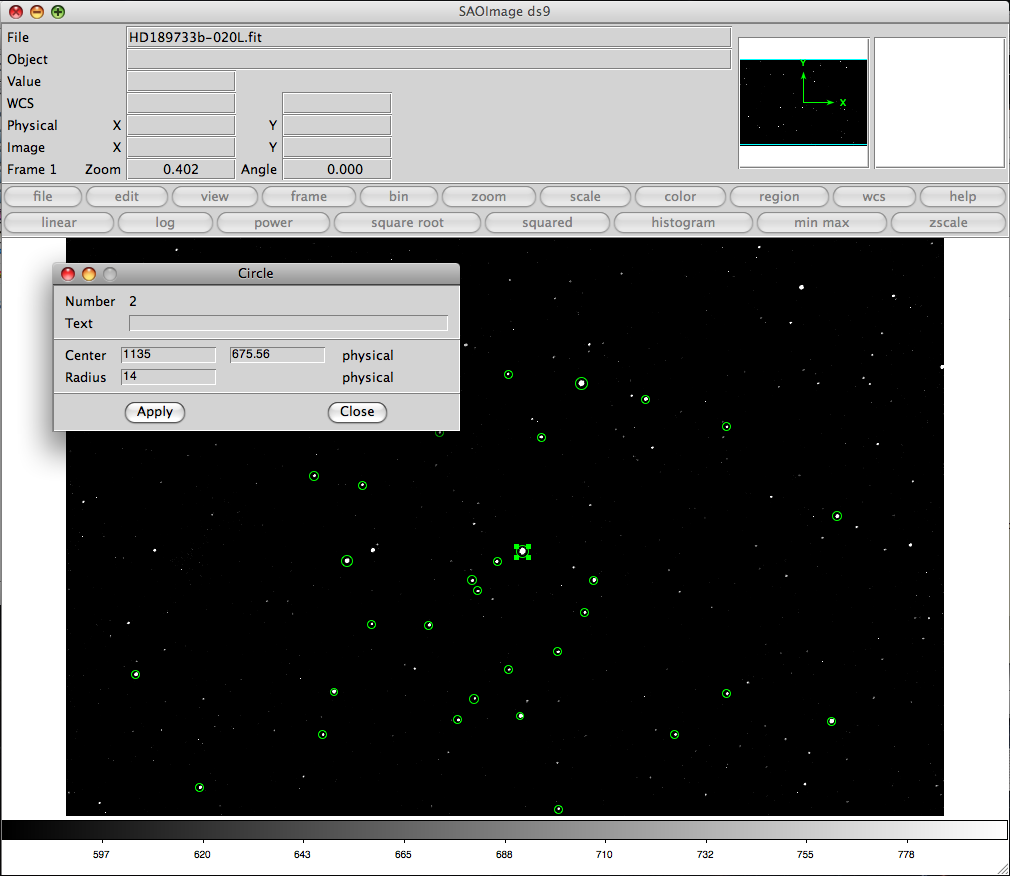
\includegraphics[scale=0.34]{imgs/ds9.png}
{\small \textbf{Screenshot 1}: Using DS9 to locate test and control stars}
\end{center}	
The first star that you select will be treated as the target star, and any subsequent choices will be comparison stars. Repeat this process for as many comparison stars as you like (try to keep it under 25 for speed). Avoid picking stars near any obvious defects on the detector, any stars less than 150 pixels from the edge of the image, or stars with a neighboring star close nearby. 

When you're done choosing control stars, go to \code{Regions} \textgreater  \code{Save Regions...} and save a regions file in a directory where you will be able to find it later. This file will contain the pixel coordinates of the stars at the beginning of the observation, which tells \oscaar which stars to track. You may want to check that the test star is in fact the first star in the regions file. Open the regions file in a text editor and check that the first line resembling ``\code{circle(100,600,10)}'' has the proper (x,y) pixel coordinates and radius (in this example, the position is (100,600) with a radius of 10). If the first circle coordinate line does not point to the target star, find the circle coordinate that does, move that line to the top of the list, and save the file.

\subsection{The Initial Parameters File: \init}

In the running directory of the code, there is a file called \init. This file is where some of your interaction with the code may happen. It is written in a unique syntax that we designed specifically for \oscaar that is intended to be a user friendly means of directing \oscaar without having to know any computer languages. 

Each line of \init is a statement of what feature you would like to turn on or off, or how you'd like to set a particular parameter. Below are explanations of all of the features you can access via \init and the arguments that they take. Once these are tweaked to your liking, you will be ready to run the code. 

\subsubsection{Locating Your Data}

	\oscaar  is built to find files by their paths. If you name the sky image files ``TrES3-001.fit," ``TrES3-002.fit" ... ``TrES3-160.fit" and name the dark frames ``dark-001.fits," ``dark-002.fits" ... ``dark-005.fits," it will be easy to set up the code to differentiate between those files. If the files are not already easily distinguishable, make them look more like the ones above now. 
	
	The first lines of \code{init.par} concern the locations of the files you will be analyzing. They are: \\ 

\indent \code{darkLoc}: The path to the dark frame files		\\
\indent \code{flatLoc}: The path to the flat field files	\\
\indent \code{imagLoc}: The path to the series of sky images for photometry	\\
\indent \code{regsLoc}: The path to the regions file from DS9 	\\

These commands expect a path as the input. For example, I could indicate where my dark frames are if they are named in the scheme from the example above with the command: \\

\indent \code{darkLoc /Users/bmorris/Desktop/Exoplanets/20110608/darks*}\\

The code will read your input just like any Unix shell, so you can use \code{*}'s, and \code{?}'s creatively to ensure that you're getting the right files for each set of images that you are trying to point to.  If you want to check that you will be pointing to the right images, you can open a Unix shell and try \\

\code{ls /the/path/you/want/to/try }\\

\noindent and see if it returns a list of the appropriate files. 

\subsubsection{Star Tracking}

The next set of options controls the star tracking algorithm. Since very well-aligned telescopes generally track imperfectly over a few hours, in most runs stars drift across the detector slightly. \oscaar  will take the initial star positions that you saved in the regions file from DS9 and track the stars as they move across the CCD using a Guassian fitting routine. 

	This bit of code is the slowest portion of the code, as fitting a 20x20 element, two dimensional Gaussian to noisy data is never an easy task. Once you do the tracking on your stars using \oscaar, you can reuse the tracking information if you need to redo the aperture photometry or differential photometry (I'll talk about those next). If you don't delete the output produced by the tracking part of the code, you won't have to run it again and spend time waiting for fits. This nifty independence of each part of the code will be a common theme in the rest of these instructions. 

	To turn the tracking algorithm on or off, simply type \code{on} or \code{off} in lower case letters after the word \textsf{track}, ie:\\
	
\indent \code{track on}\\

	And it's as simple as that. If you'd like to see how the code works a little deeper or troubleshoot a problem that you think might be related to tracking, you may want to see a plot of the Gaussian fitting as it is performed. If you are adventurous and would like to try it, throw in\\

\indent \code{trackplot on}\\

The resulting plots are three dimensional and can be rotated and manipulated. The red wire-frame is the data and the blue surface is the fit. 

	In order to help the fitting algorithm find the object faster, enter an estimate for the sigma parameter, corresponding to the radial width of the star in pixels, using the \textsf{estsig} parameter: \\
	
\indent \code{estsig 2.0}\\

If you try to start a run and the fitting algorithm is barfing errors like those shown in Section~\ref{sec:err}, you likely need to pick a new \textsf{estsig} value. 

\subsubsection{Aperture Photometry}

In this documentation I've talked about ``aperture photometry" and ``differential photometry" as if they are different things that are intimately related. Aperture photometry is the process of looking at the intensity of a star by determining the flux through a digital aperture. Differential photometry is the process of taking instrumental magnitudes obtained from aperture photometry of different stars, averaging them and comparing them to another star to look for variation of one star over time. This section will briefly discuss using the algorithm that does the aperture photometry.

	Let's turn on the aperture photometry algorithm:\\
	
\indent \code{aper on}\\

	The fit produced in the star tracking stage has two important output values: an (x,y) pixel coordinate for the center of the star and a $ \sigma $ parameter determining the radial width of that star. The code will consider a ``source" and ``sky" aperture around the star based on a scaling parameter that you enter. The default is to make a source aperture 5.5 the $ \sigma $ of the source, so let's set this aperture radius:\\
	
	\indent \code{aprad 5.5}\\
	
	Just in case one of the control stars was too close to saturating the CCD, there is an extra check built in to the code to ignore stars more than 85\% of the saturation limit. Since each CCD could have a different saturation count limit, you can enter the limit on your detector into the \code{init.par} file as follows for a CCD with a 60,000 count limit: \\
	
\indent \code{satur 60000} \\

	If you were to try to compare photometry between different CCDs, you would need to keep track of the different gains (sometimes represented as a ``K") of each device. In order to make the measurements as consistent as possible across different devices, there is a gain parameter for you to specify. If you do not know the gain for your device, look at the header information of any of your FITS files recorded by this device. The gain is noted in the ``EGAIN" field. For my SBIG ST-10, I'll set it to:\\
	
\indent \code{Kccd 0.7799} \\

\noindent Note the upper case \code{K}, this is the only in the upper case letter in the \code{init.par} file. 

	Similar to the tracking algorithm options, there is an aperture photometry option for displaying all plots. This is not recommended for common use, but if you need to troubleshoot a problem or check that your aperture radius is appropriate, you may want to see a few plots controlled by the \code{aperplot} parameter. These plots will show each star as the aperture photometry algorithm is being applied to it, along with two red circles representing the source aperture radius (controlled by \code{aprad}) and an outer circle showing the sky aperture between the source radius and some further radius that will be used to find the background intensity. To turn on these plots:\\

\indent \code{aperplot off}\\


\subsubsection{Differential Photometry}

Finally it is time to tell \oscaar  to do the differential photometry. The differential photometry algorithm is activated with \\

\indent \code{diff on}\\

\noindent which calculates the magnitude of the test star with respect to the control stars. The process is repeated to compare each control star against all of the other control stars, as well. This way you can visually inspect the control stars to make sure they aren't variable. 

All that's left to do now is to visualize the data!  Turn on the built-in GUI with\\

\indent \code{diffgui on}\\

\noindent Instructions for using the GUI can be found in Section~\ref{sec:gui}. \\


\subsection{Initializing \oscaar}

\code{init.par} is now all set up. \oscaar  is ready to run! To run oscaar, open a Unix shell and change directories to the oscaar directory. Execute the Python script that controls \oscaar : \\

\indent \code{\$ python photom15.py} \\

\noindent This file is specific to \code{oscaar1.1.0}. Different versions have ``photom.py" files with different numbers. 

When the code is running, the following will be printed to standard out: \\

{\addtolength{\leftskip}{10 mm}
{\scriptsize
\noindent \code{Loading and averaging dark frames...\\
IMAGE 1/353, STAR 1/3************************\\
\{'amp': 20953, 'sigma': 2, 'xcenter': 15, 'ycenter': 13, 'offset': 435\}\\
IMAGE 1/353, STAR 2/3************************\\
\{'amp': 1143, 'sigma': 2, 'xcenter': 9, 'ycenter': 8, 'offset': 391\}\\
IMAGE 1/353, STAR 3/3************************\\
\{'amp': 591, 'sigma': 2, 'xcenter': 9, 'ycenter': 9, 'offset': 390\} } \\
 \vdots

	}
}

For each star, the \oscaar  runs the tracking algorithm and prints the output from the Gaussian fit, then runs the aperture photometry algorithm. The important fit parameters are displayed so you can check that they are reasonable while the code is running. Here the values are abbreviated as integers for clarity, though they will appear as long decimals (``floats'' in Python speak) in your standard out. 

\subsubsection{Recognizing Errors}
\label{sec:err}
Sometimes the script will return something resembling the following: \\

{\addtolength{\leftskip}{10 mm}
{\scriptsize
\noindent \code{IMAGE 76/353, STAR 2/3************************ \\
eigenvalues: \\
-0.0322264\\
0.631025\\
0.960443\\
1.12215\\
2.31861\\
matrix forced pos-def by adding 0.034545 to diagonal \\
\{'amp': 1757, 'sigma': 1, 'xcenter': 11, 'ycenter': 9, 'offset': 324\} }\\

	}
}

\noindent This indicates that the fitting algorithm had some difficulty, but it eventually found the proper fit. It is OK if this happens in bursts as \oscaar  analyses a bad image, as long as the output eventually looks normal again. 

It is \textbf{not} OK if the following is printed: \\

{\addtolength{\leftskip}{10 mm}
{\scriptsize
\noindent \code{IMAGE 1/353, STAR 1/3*********************** \\
\vdots \\
invalid value encountered in double\_scalars\\
MnHesse: 2nd derivative zero for parameter 0\\
MnHesse fails and will return diagonal matrix \\
MnHesse: 2nd derivative zero for parameter 0\\
MnHesse fails and will return diagonal matrix \\
ERROR: Fit not found for this frame.}\\

	}
}

\noindent As mentioned earlier, if you choose a bad \code{estsig} value in the \code{init.par} file, this error may be the fitting algorithm dying as a result. 

	If a star is not located where the \code{Regions} file tells \oscaar  to look, the fitting algorithm will fail with the error above. If this happens you should kill the script with \code{Ctrl+C}. Open your \code{Regions} file in DS9 and check that the star that failed is properly marked, and open the image where the code failed and look for irregularities (like a plane or satellite passing in the image, the tracking on your telescope dying, the star running off the edge of the detector, etc.).

If the image is bad for any reason, you can rename that image so that it no longer matches what the \code{init.par} file is looking for and it gets skipped over. Then start the script again. If you do this to many consecutive images, the tracking algorithm might not be able to track the stars before and after the break. If this is the case, you may need to do the \oscaar  analysis in separate chunks with unique \code{Regions} files corresponding to before and after the break. 

If you can't find anything that seems to be wrong, it is best to discontinue use of this control star. Open the regions file, go to the \code{circle(x,y,r)} line corresponding to the failed star and comment it out with a preceding \code{\#}: \\

\indent \code{\#circle(x,y,r)}\\

\subsection{Using the \oscaar  GUI} 
\label{sec:gui}

When \code{diffgui} is \code{on}, the built-in GUI for \oscaar  will open with your data. This can be explicitly triggered from the command line with \\

\indent \code{\$ python differgui2.py}\\

\noindent in \code{oscaar1.1.0}. The following interface will be displayed:\\

\begin{center}
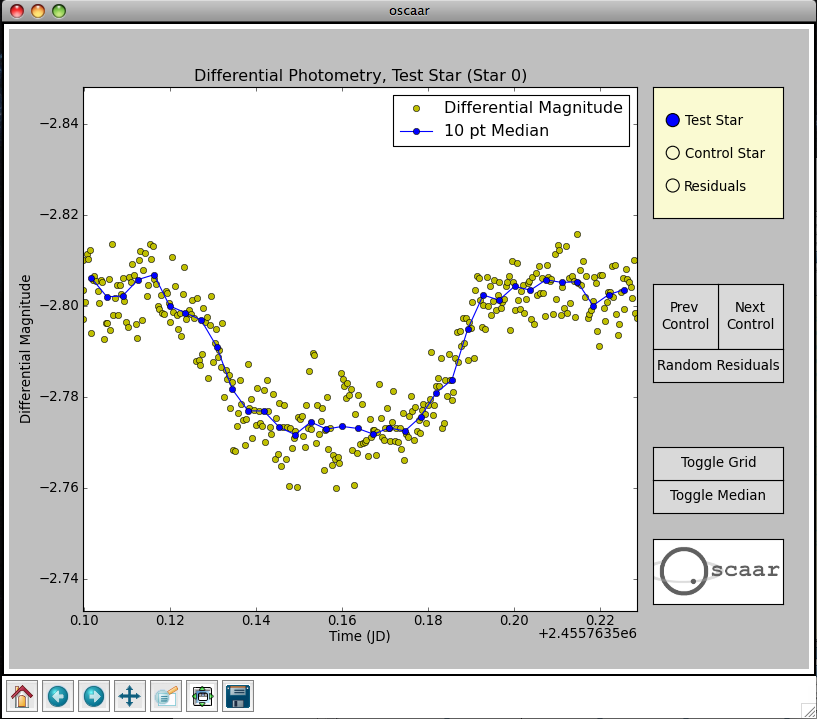
\includegraphics[scale=0.4]{imgs/gui1.png}
{\small \textbf{Screenshot 2}: The starting view in \oscaar 's GUI}
\end{center}
\bigskip

This shows the light curve of your test star. The example in Screenshot 2 is a light curve of transit of exoplanet HD 189733b. The vertical axis corresponds to the differential magnitude of the star with some constant arbitrary vertical displacement. Note that the dimmer astronomical magnitudes correspond to larger numbers. The horizontal axis is time in Julian Date, as recorded in the FITS header of your test star. 

This plot is interactive. You can click on the middle button at the bottom of the window (the axes icon) to select a panning tool. The magnifying glass icon is a rectangular zoom tool. Click the home icon to return to the initial (default) view. Click the floppy disk icon to save the image to a PNG. 

You can check for intrinsic variability in your control stars by clicking the ``Control Star'' button in the yellow box in the upper right. You can go through all of the control stars by clicking the ``Prev Control'' and ``Next Control'' buttons.  \\

\begin{center}
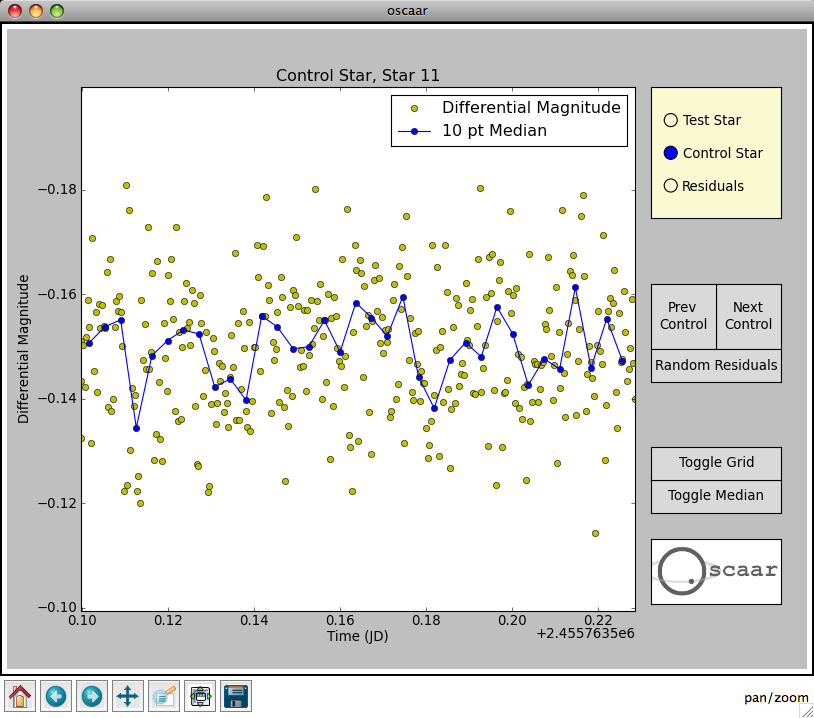
\includegraphics[scale=0.4]{imgs/gui2.png}
{\small \textbf{Screenshot 3}: Checking control stars in \oscaar 's GUI }
\end{center}
\bigskip

Even good control stars will show noise like this one. The scaling of the magnitude axis changes from star to star, so even though they may all look similar, the scale is almost certainly changing. 

The ``Residuals'' plots may be a bit of a misnomer. They represent the difference between the differential magnitude measurements of two random control stars. This is mainly a tool for troubleshooting. If there are big, discontinuous jumps in these ``Residual'' plots or trends in the data apart from noise around zero, there is likely something wrong with the analysis of that control star. To check different pairs of stars, click ``Random Residuals''. 

Grid lines and the median binning can be toggled with the ``Toggle Grid'' and ``Toggle Median'' buttons. 


\section{\oscaar For Programmers} \label{sec:api}

\subsubsection{Navigating \oscaar  Output Files}

\oscaar  outputs files into different directories within the \code{oscaar1.1.0} running directory. \\


\begin{center}
\begin{tabular*}{\textwidth}{c  c  c }
\hline
\hline
\textbf{Directory} & \textbf{Contents} & \textbf{Contents Format}\\\hline \\

filelists & Names of files that \oscaar  will need & List of paths \\ \\
aper\_out & Aperture photometry results & Inst. mag., error  \\ \\
track\_out & Tracking algorithm results & x-pos., y-pos., sigma\\ \\
diff\_out & Differential photometric magnitude & Diff. mag., error  \\  \\
time\_out & JD time extracted from test star headers & List of JD \\ \\
\hline \\
\end{tabular*} \\
\textbf{Note}: The differential magnitude error algorithm is still not well refined. 
\end{center}
\bigskip 

\noindent The \oscaar  running directory is intended to be copied for each new run you do to preserve the running parameters for your records. If you start a new run in an \oscaar  directory with these output directories already generated, \oscaar  will ask you before overwriting them. 


\subsubsection{\oscaar  API}

You are welcome to write your own script that reads the different output files, and manipulates the data however you like. This will give you the power to script any analysis you can think of. The script that does the differential photometry in \code{oscaar1.1.0} is \code{differcalc2.py}. It uses object orientation to manage all of the different bits of data that are involved. The classes used in \code{differcalc2.py} are defined in \code{diffmodule3.py}, and you may find them useful to handle the myriad of data elements. 

For example, the sample script below will plot the pixel coordinates of the test star throughout the run by objectively accessing the x and y positions of the star: \\

{\addtolength{\leftskip}{10 mm}
{\scriptsize
\noindent \code{import matplotlib.pyplot as plt \\
import diffmodule3 as dm \#\# Classes for "fluxArray" and "starObj" \\ 
\\
teststar = dm.starObj(`001') \#\# Initialize a star object \\ 
x = teststar.trackx()      \#\# Access the x and y positions \\
y = teststar.tracky() \\
\\
plt.plot(x,y)                \#\# Plot the star positions \\
plt.title(`Pixel Coordinates of the Test Star') \\
plt.show() }\\

	}
}

\noindent which may produce a plot that looks something like this: \\

\begin{center}
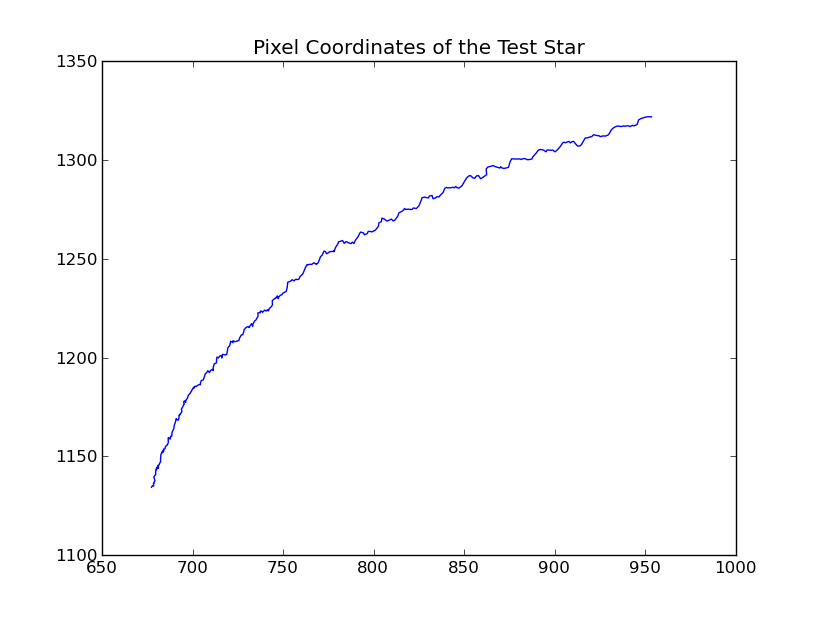
\includegraphics[scale=0.5]{imgs/sample.png} \\
{\small \textbf{Screenshot 4}: Making a quick script to see the star position on the detector throughout the run}
\end{center}
\bigskip

\noindent Open up an interactive Python shell, import the module and do a \code{help(differmodule3)} to see all of the available object classes and methods. 



\subsection{Contributing to \oscaar}
This version of \oscaar was made by four people, and we're proud of the work we've done. But \oscaar can still be improved and we need your help! \oscaar is used in more than 10 countries by amateurs and professionals alike, and in order to keep up with the demands of providing a user-friendly differential photometry code for an international audience, we'd love to have your help if you can: code in Python, translate some documentation, or provide any feedback at all. If you'd like to help, please contact us at \href{mailto:oscaarUMD@gmail.com}{oscaarUMD@gmail.com}. 




\section{Acknowledgements}
\oscaar has come a long way from the first 1,000 lines of code that Brett Morris wrote in 2011. It could not have gotten there without the help of the following colleagues: 
Harley Katz, Drake Deming, Elizabeth Warner, Alberto Bolatto, Avi Mandell, Jacob Endres, Daniel Galdi, Sam Gross.

	
\end{document}